\chapter{Từ các lượng tử của dây mở đến tachyon và hấp dẫn}

\lectureoverview{Giờ đây ta lượng tử hóa các mode chuẩn tìm được trong bài giảng trước và hỏi chúng tạo ra những trạng thái hạt nào. Mỗi mode ngang là một dao động tử điều hòa, nhưng chuẩn hóa của nó hơi khác thường: kích thích mode \(n\) làm tăng năng lượng light-front, và do đó cả mức bình phương khối lượng, thêm \(n\) đơn vị. Mức kích thích thứ nhất của dây mở biến đổi đúng như hai phân cực ngang của một vectơ không khối lượng. Vì thế, tính nhất quán tương đối tính buộc bình phương khối lượng của trạng thái cơ bản phải âm. Trạng thái đó là tachyon của dây boson; ý nghĩa thực sự của nó là một chân không không ổn định, chứ không phải một hạt siêu quang thực tế. Cuối cùng, một khi các dây tương tác, sự nối và tách khiến dây kín trở nên không thể tránh khỏi; kích thích thấp nhất của dây kín sẽ là graviton.}

\section{Dao động tử ẩn trong mỗi mode dây}

Đối với một tọa độ ngang \(X\), mode chuẩn khác không thứ \(n\) có năng lượng và Lagrangian

\begin{align}
  E_n
  &=
  \frac14\dot X_n^{\,2}
  +\frac{n^2}{4}X_n^2,
  \label{eq:l03-mode-energy}\\
  L_n
  &=
  \frac14\dot X_n^{\,2}
  -\frac{n^2}{4}X_n^2.
  \label{eq:l03-mode-lagrangian}
\end{align}

Các thừa số \(1/4\) không phải là lỗi. Chúng ghi lại chuẩn hóa đã được chọn khi tác dụng của dây được rút gọn thành các mode Fourier độc lập. Vì vậy, bước đầu tiên trong việc xây dựng Hamiltonian là tính xung lượng chính tắc,

\begin{equation}
  p_n=\frac{\partial L_n}{\partial\dot X_n}
     =\frac12\dot X_n,
  \qquad
  \dot X_n=2p_n.
  \label{eq:l03-canonical-momentum}
\end{equation}

Phép biến đổi Legendre cho

\begin{equation}
  H_n=p_n\dot X_n-L_n
     =p_n^2+\frac{n^2}{4}X_n^2.
  \label{eq:l03-mode-hamiltonian}
\end{equation}

\begin{figure}[H]\centering
  \includegraphics[width=0.82\textwidth]{lecture_03_figure_01.png}\caption{Năng lượng mode, Lagrangian, xung lượng chính tắc và Hamiltonian trong chuẩn hóa thừa hưởng từ dây mở.}\lectureframe{00:05:40}\label{fig:l03-mode-hamiltonian-board}\end{figure}

Để phân tích \(H_n\) thành nhân tử, hãy kết hợp \(X_n\) và \(p_n\) thành

\begin{equation}
  \frac{nX_n}{2}\pm i p_n.
\end{equation}

Về cổ điển, hai nhân tử sẽ giao hoán, nhưng về lượng tử thì

\begin{equation}
  [X_n,p_m]=i\delta_{nm}
  \label{eq:l03-canonical-commutator}
\end{equation}

trong đơn vị với \(\hbar=1\). Các hạng chéo không triệt tiêu một cách vô hại. Với một mode cố định,

\begin{align}
  \left[\frac{nX_n}{2}+ip_n,
        \frac{nX_n}{2}-ip_n\right]
  &=n,
  \label{eq:l03-unscaled-commutator}\\
  \left(\frac{nX_n}{2}-ip_n\right)
  \left(\frac{nX_n}{2}+ip_n\right)
  &=H_n-\frac n2.
  \label{eq:l03-factorized-hamiltonian}
\end{align}

\begin{figure}[H]\centering
  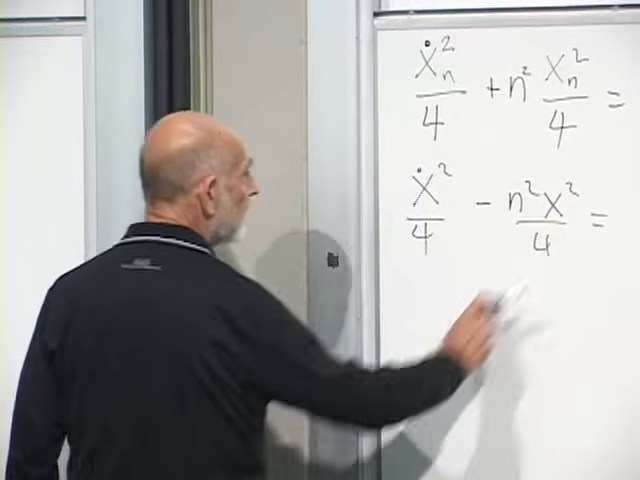
\includegraphics[width=0.82\textwidth]{lecture_03_figure_02.png}\caption{Phép tính trên bảng, trong đó giao hoán tử chính tắc cung cấp thừa số \(n\).}\lectureframe{00:10:30}\label{fig:l03-commutator-board}\end{figure}

Thừa số \(n\) chỉ ra cách chuẩn hóa các toán tử nâng hạ:

\begin{align}
  a_n
  &\equiv
  \frac{\sqrt n}{2}X_n+\frac{i}{\sqrt n}p_n,
  \label{eq:l03-annihilator}\\
  a_n^\dagger
  &\equiv
  \frac{\sqrt n}{2}X_n-\frac{i}{\sqrt n}p_n.
  \label{eq:l03-creator}
\end{align}

Chúng thỏa mãn

\begin{equation}
  [a_n,a_m^\dagger]=\delta_{nm},
  \qquad
  H_n=n\left(a_n^\dagger a_n+\frac12\right).
  \label{eq:l03-oscillator-algebra}
\end{equation}

Vì vậy, \(a_n^\dagger\) thêm một lượng tử vào dao động tử thứ \(n\), nhưng lượng tử đó mang \(n\) đơn vị năng lượng mode. Khoảng cách mức quen thuộc của dao động tử không hề mất đi; tần số của nó là \(\omega_n=n\).

\begin{figure}[H]\centering
  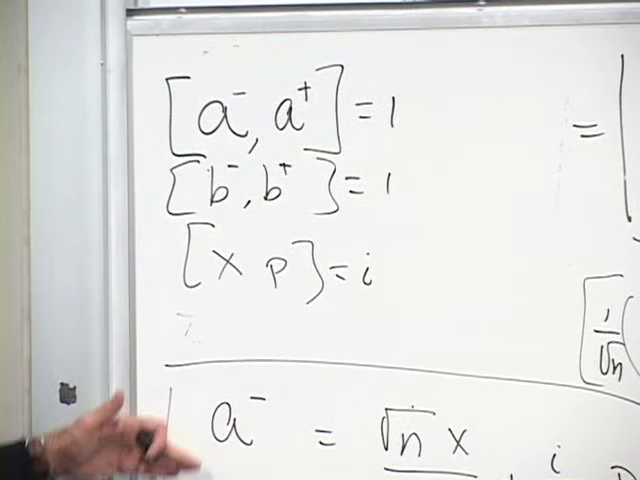
\includegraphics[width=0.82\textwidth]{lecture_03_figure_03.png}\caption{Các toán tử hủy và tạo đã được chuẩn hóa cho dao động tử dây thứ \(n\).}\lectureframe{00:12:00}\label{fig:l03-ladder-board}\end{figure}

\subsection{Hai tháp dao động ngang}

Trong không-thời gian 4 chiều, một dây mang động lượng rất lớn dọc theo trục \(z\) có hai tọa độ ngang, \(X\) và \(Y\). Vì vậy ta cần hai tháp dao động tử độc lập. Cho \(a_n,a_n^\dagger\) tác dụng lên các mode \(X\) và \(b_n,b_n^\dagger\) tác dụng lên các mode \(Y\). Giải \eqref{eq:l03-annihilator}--\eqref{eq:l03-creator} theo các tọa độ, ta được

\begin{equation}
  X_n=\frac{a_n+a_n^\dagger}{\sqrt n},
  \qquad
  Y_n=\frac{b_n+b_n^\dagger}{\sqrt n}.
  \label{eq:l03-mode-coordinates}
\end{equation}

\begin{figure}[H]\centering
  \includegraphics[width=0.78\textwidth]{lecture_03_figure_04.png}\caption{Biểu diễn một tọa độ mode theo các toán tử tạo và hủy của nó.}\lectureframe{00:17:05}\label{fig:l03-coordinate-operator-board}\end{figure}

Các tọa độ của dây mở được khai triển theo các mode Neumann,

\begin{align}
  X(\sigma,\tau)
  &=X_{\rm cm}(\tau)
    +\sum_{n=1}^{\infty}X_n(\tau)\cos(n\sigma),
  \label{eq:l03-X-fourier}\\
  Y(\sigma,\tau)
  &=Y_{\rm cm}(\tau)
    +\sum_{n=1}^{\infty}Y_n(\tau)\cos(n\sigma).
  \label{eq:l03-Y-fourier}
\end{align}

Các hàm cos xuất hiện vì độ dốc tại các đầu mút triệt tiêu. Thay \eqref{eq:l03-mode-coordinates} vào sẽ biến chính dây thành một toán tử:

\begin{align}
  X(\sigma,\tau)
  &=X_{\rm cm}(\tau)
    +\sum_{n=1}^{\infty}
      \frac{a_n(\tau)+a_n^\dagger(\tau)}{\sqrt n}
      \cos(n\sigma),
  \label{eq:l03-X-operator}\\
  Y(\sigma,\tau)
  &=Y_{\rm cm}(\tau)
    +\sum_{n=1}^{\infty}
      \frac{b_n(\tau)+b_n^\dagger(\tau)}{\sqrt n}
      \cos(n\sigma).
  \label{eq:l03-Y-operator}
\end{align}

\begin{figure}[H]\centering
  \begin{minipage}[t]{0.48\textwidth}\centering
    \includegraphics[width=\textwidth]{lecture_03_figure_05.png}\par\smallskip\footnotesize (a) Khai triển tọa độ theo mode.\end{minipage}\hfill
  \begin{minipage}[t]{0.48\textwidth}\centering
    \includegraphics[width=\textwidth]{lecture_03_figure_06.png}\par\smallskip\footnotesize (b) Các toán tử nâng hạ được thế vào các tọa độ dây.\end{minipage}\caption{Hình dạng của dây mở lượng tử được ghép lại từ tất cả các toán tử dao động ngang của nó.}\lectureframe{00:20:35 and 00:21:05}\label{fig:l03-string-coordinate-board}\end{figure}

\begin{classroomqa}\audiencequestion{Liệu \(X_n\) cũng là một hàm của \(\sigma\) không?\lecturetimestamp{00:21:48}}\lecturerresponse{Không. Sự phụ thuộc vào \(\sigma\) nằm hoàn toàn trong \(\cos(n\sigma)\). Hệ số \(X_n\) là biên độ phụ thuộc thời gian của mẫu không gian đó, nên \(X_n=X_n(\tau)\).}\end{classroomqa}

\begin{classroomqa}\audiencequestion{Vì sao các toán tử được gọi là nâng và hạ dường như lại có dấu ngược nhau?\lecturetimestamp{00:23:13}}\lecturerresponse{Dấu nhìn thấy được của \(ip_n\) không phải là quy tắc đặt tên. Hãy tính giao hoán tử với Hamiltonian. Toán tử thỏa mãn \([H_n,a_n^\dagger]=n a_n^\dagger\) làm tăng năng lượng; toán tử thỏa mãn \([H_n,a_n]=-n a_n\) làm giảm nó.}\end{classroomqa}

Bức tranh hai tháp ngang chỉ là một minh họa sư phạm trong 4 chiều. Một dây boson được lượng tử hóa nhất quán có 26 chiều không-thời gian, nên nó có 24 họ dao động tử ngang chứ không phải 2. Logic bên dưới không thay đổi: số trạng thái ở mức thứ nhất phải khớp với số phân cực vật lý của một vectơ không khối lượng trong cùng số chiều.

\section{Spin của hạt có khối lượng và helicity của hạt không khối lượng}

Trước khi gán spin cho các trạng thái dây, ta cần một sự phân biệt rành mạch. Một hạt có khối lượng với spin \(J\) có \(2J+1\) trạng thái spin,

\begin{equation}
  m_J=-J,-J+1,\ldots,J-1,J.
  \label{eq:l03-massive-spin-multiplet}
\end{equation}

Ví dụ, một hạt spin 1 có khối lượng có 3 phân cực và một hạt spin 2 có khối lượng có 5 phân cực. Ta có thể thấy vì sao bằng cách chuyển sang hệ quy chiếu nghỉ. Ở đó mọi phép quay không gian đều khả dụng. Xoay trục spin, boost trở lại, và mọi thành phần \(2J+1\) đều thuộc về cùng một hạt tương đối tính.

Một hạt không khối lượng không có hệ quy chiếu nghỉ. Nhãn spin bất biến của nó là helicity, tức mômen góc dọc theo hướng chuyển động. Photon chỉ có \(h=+1\) và \(h=-1\); graviton chỉ có \(h=+2\) và \(h=-2\). Một vô hướng có một trạng thái \(h=0\). Bài giảng dùng đối xứng phản xạ để ghép cặp hai helicity. Trong một lý thuyết chiral, một biểu diễn bất khả quy không khối lượng đơn lẻ có thể chỉ mang một helicity, nên việc ghép cặp là một phát biểu đối xứng bổ sung chứ không phải hệ quả chỉ riêng của tính không khối lượng.\editorialnote{Phân loại little group hiện đại cho phép các biểu diễn không khối lượng một-helicity. Tính chẵn lẻ hoặc một nội dung trường đầy đủ CPT thích hợp cung cấp helicity đối ngược trong các ví dụ photon và graviton quen thuộc.}

\begin{figure}[H]\centering
  \begin{minipage}[t]{0.45\textwidth}\centering
    \includegraphics[width=\textwidth]{lecture_03_figure_07.png}\par\smallskip\footnotesize (a) Phép đếm trạng thái spin được bắt đầu trên bảng.\end{minipage}\hfill
  \begin{minipage}[t]{0.5\textwidth}\centering
    \begin{adjustbox}{max width=\linewidth}\begin{tabular}{@{}ccc@{}}\toprule
      Spin &Trạng thái có khối lượng &Helicity không khối lượng \\\midrule
      \(0\) & \(1\) & \(0\) \\\(1\) & \(3\) & \(+1,-1\) \\\(2\) & \(5\) & \(+2,-2\) \\\bottomrule
    \end{tabular}\end{adjustbox}\end{minipage}\caption{Khối lượng tước đi hệ quy chiếu nghỉ và cùng với nó là các hình chiếu spin trung gian.}\lectureframe{00:27:40}\label{fig:l03-spin-count}\end{figure}

\subsection{Phân cực photon tuyến tính và tròn}

Xét một photon chuyển động dọc theo \(z\). Hai phân cực tuyến tính ngang của nó là \(\ket{x}\) và \(\ket{y}\). Chúng không phải là các trạng thái riêng helicity. Các trạng thái phân cực tròn là

\begin{align}
  \ket{R}
  &=\frac{1}{\sqrt2}\left(\ket{x}+i\ket{y}\right),
  \label{eq:l03-right-circular}\\
  \ket{L}
  &=\frac{1}{\sqrt2}\left(\ket{x}-i\ket{y}\right),
  \label{eq:l03-left-circular}
\end{align}

với helicity \(+1\) và \(-1\), tùy theo quy ước dùng để gọi phải và trái. Một photon phân cực tuyến tính là chồng chập của hai kết cục đó. Helicity trung bình của nó có thể triệt tiêu, nhưng một phép đo helicity không bao giờ tìm thấy một photon spin 0. Tương tự,

\begin{equation}
  \frac{1}{\sqrt2}\left(\ket{x}+\ket{y}\right)
\end{equation}

đơn giản là phân cực tuyến tính ở góc 45 độ.

\begin{figure}[H]\centering
  \begin{minipage}[t]{0.48\textwidth}\centering
    \includegraphics[width=\textwidth]{lecture_03_figure_08.png}\par\smallskip\footnotesize (a) Các trạng thái phân cực tròn trên bảng.\end{minipage}\hfill
  \begin{minipage}[t]{0.48\textwidth}\centering
    \begin{adjustbox}{max width=\linewidth}\begin{tikzpicture}[>=Latex,scale=0.9]
      \draw[->,thick] (0,0) -- (3.4,0) node[right] {\(z\)};
      \draw[->,blue!70!black,thick] (0,0) -- (0,2.0)
        node[above] {\(x\)};
      \draw[->,orange!85!black,thick] (0,0) -- (-1.4,-1.2)
        node[below left] {\(y\)};
      \draw[red!70!black,thick,->]
        plot[domain=0:320,samples=80]
        ({1.0*cos(\x)},{0.58*sin(\x)+0.4});
      \node[red!70!black] at (1.55,1.25) {circular};
    \end{tikzpicture}\end{adjustbox}\end{minipage}\caption{Phân cực tuyến tính cung cấp một cơ sở ngang; các tổ hợp tròn chéo hóa helicity.}\lectureframe{00:37:45}\label{fig:l03-polarization}\end{figure}

\begin{classroomqa}\audiencequestion{Điều này có giống sự tách các trạng thái spin trong thí nghiệm Stern--Gerlach không?\lecturetimestamp{00:37:40}}\lecturerresponse{Ý tưởng chồng chập lượng tử là như nhau, nhưng đối với photon thì ngôn ngữ trực tiếp là phân cực. Một phép đo phân cực tròn phân biệt hai helicity; không có photon dọc spin 0 nào trong chùm.}\end{classroomqa}

Graviton lặp lại mô thức đó ở spin 2. Để theo dõi spin, ta có thể viết một cách sơ đồ

\begin{equation}
  \ket{+2}\sim\ket{+1}\otimes\ket{+1},
  \qquad
  \ket{-2}\sim\ket{-1}\otimes\ket{-1}.
  \label{eq:l03-graviton-helicity}
\end{equation}

Điều này không có nghĩa là graviton theo nghĩa đen được tạo thành từ hai photon. Nó nói rằng hai helicity bằng nhau cộng lại cho helicity spin-2 đúng.

\begin{classroomqa}\audiencequestion{Phép tương tự hai photon có mở rộng sang các số lượng tử khác không?\lecturetimestamp{00:41:05}}\lecturerresponse{Không, nếu hiểu như một mô hình thành phần. Có những công thức mạnh, trong đó các biên độ hấp dẫn trông như tích, hay ``bình phương'', của các biên độ lý thuyết chuẩn, nhưng graviton vẫn là hạt riêng của nó. Phép tương tự đáng tin nhất ở đây là như một phát biểu về helicity.\editorialnote{Các quan hệ Kawai--Lewellen--Tye hiện đại và các quan hệ double-copy làm cho phát biểu về biên độ trở nên chính xác trong những lý thuyết thích hợp; chúng không biến graviton thành trạng thái liên kết của hai photon.}}\end{classroomqa}

\begin{classroomqa}\audiencequestion{Một photon có thể có bất kỳ động lượng nào, vậy chẳng phải nó có phổ liên tục thay vì phổ cô lập vốn được yêu cầu đối với một hạt sao?\lecturetimestamp{00:42:17}}\lecturerresponse{Biến liên tục là động lượng tâm khối. Giữ cố định động lượng đó và xét khối lượng bất biến nội tại. Một hạt được nhận diện bởi một mức khối lượng cô lập; rồi việc biến thiên động lượng toàn phần của nó tạo ra quan hệ tán sắc liên tục quen thuộc.}\end{classroomqa}

\enlargethispage{1pt}
\section{Các mức thấp nhất của dây mở}

Giờ ta có thể quay lại dây. Trong mô tả động lượng lớn, năng lượng light-front nội tại hữu hạn tỉ lệ với bình phương khối lượng bất biến. Tạm bỏ qua thang dây tổng thể, hãy viết phổ là

\begin{equation}
  \begin{aligned}
    M^2
    &=m_0^2
      +\sum_{n=1}^{\infty}n
       \left(N_n^{(a)}+N_n^{(b)}\right),\\
    N_n^{(a)}&=a_n^\dagger a_n,
    \qquad
    N_n^{(b)}=b_n^\dagger b_n.
  \end{aligned}
  \label{eq:l03-open-spectrum}
\end{equation}

Trạng thái cơ bản của các dao động tử thỏa mãn

\begin{equation}
  a_n\ket{0}=0,
  \qquad
  b_n\ket{0}=0,
  \qquad n=1,2,\ldots .
  \label{eq:l03-ground-annihilation}
\end{equation}

Đó không phải là sự vắng mặt trống rỗng của dây. Đó là dây lượng tử ít kích thích nhất, và các tọa độ của nó vẫn dao động. Gọi bình phương khối lượng của nó là \(m_0^2\), chưa được xác định.

\begin{figure}[H]\centering
  \includegraphics[width=0.78\textwidth]{lecture_03_figure_09.png}\caption{Trạng thái cơ bản của dây mở và các điều kiện hủy xác định nó.}\lectureframe{00:45:20}\label{fig:l03-ground-state-board}\end{figure}

Các kích thích ít tốn năng lượng nhất dùng các toán tử tạo \(n=1\):

\begin{equation}
  a_1^\dagger\ket{0},
  \qquad
  b_1^\dagger\ket{0},
  \qquad
  M^2=m_0^2+1.
  \label{eq:l03-first-level}
\end{equation}

\begin{figure}[H]\centering
  \includegraphics[width=0.78\textwidth]{lecture_03_figure_10.png}\caption{Một trong hai trạng thái bậc nhất suy biến, với phần tăng của bình phương khối lượng được viết trên bảng.}\lectureframe{00:49:25}\label{fig:l03-first-level-board}\end{figure}

Số ``một'' trong eqref{eq:l03-first-level} không phải là một joule, một electron volt hay một khối lượng Planck. Ta đã lược bỏ thang dây có thứ nguyên. Hiện thời, nó có nghĩa là một bậc trên thang bình phương khối lượng của dao động tử; các đơn vị còn thiếu sẽ được phục hồi trong bài giảng tiếp theo.

Mọi tổ hợp tuyến tính của hai trạng thái suy biến ấy cũng là một trạng thái ở mức này. Cụ thể,

\begin{equation}
  \frac{1}{\sqrt2}
  \left(a_1^\dagger\pm i b_1^\dagger\right)\ket{0}
  \label{eq:l03-string-circular-states}
\end{equation}

là phép tương tự trong dây của phân cực tròn. Dưới một phép quay trong mặt phẳng \(x\)-\(y\), \(a_1^\dagger\) và \(b_1^\dagger\) biến đổi như hai thành phần của một vectơ ngang. Vì thế các tổ hợp trong \eqref{eq:l03-string-circular-states} có helicity \(+1\) và \(-1\).

\begin{figure}[H]\centering
  \includegraphics[width=0.82\textwidth]{lecture_03_figure_11.png}\caption{Các điều kiện trạng thái cơ bản, hai kích thích bậc nhất và các tổ hợp tròn của chúng được tập hợp trên bảng.}\lectureframe{00:56:00}\label{fig:l03-level-structure-board}\end{figure}

Không có trạng thái suy biến thứ ba nào có thể đóng vai trò là một phân cực dọc. Nếu hai trạng thái này có khối lượng khác không, thì một hạt tương đối tính spin một sẽ cần ba phân cực. Với đúng hai phân cực, trạng thái đó phải không khối lượng. Do đó

\begin{equation}
  m_0^2+1=0,
  \qquad
  m_0^2=-1.
  \label{eq:l03-intercept-condition}
\end{equation}

Mức thứ nhất giống photon: đó là một trạng thái vectơ chuẩn không khối lượng. Nó không nhất thiết là photon của điện từ học; bản sắc chuẩn cuối cùng của nó phụ thuộc vào mô hình dây. Trạng thái cơ bản bên dưới nó có bình phương khối lượng âm. Đó là tachyon của dây mở boson.\editorialnote{Trong dây boson tới hạn đầy đủ, độ chặn do sắp thứ tự chuẩn và đại số Lorentz gắn với \(D=26\). Phép tính của bài giảng với hai hướng ngang là cái bóng 4 chiều của cùng một lập luận đếm trạng thái: \(D-2\) trạng thái dao động tử ở mức thứ nhất khớp với \(D-2\) phân cực vật lý của một vectơ không khối lượng.}

\begin{classroomqa}
\audiencequestion{Vì sao chúng ta phải quan tâm đến việc \(m_0^2\) âm?\lecturetimestamp{00:56:35}}
\lecturerresponse{Vì bình phương khối lượng là độ cong của thế trường bậc hai quanh trạng thái mà ta đã gọi là chân không. Độ cong âm có nghĩa là cấu hình này không phải là một trạng thái nền ổn định. Phép tính tiếp theo sẽ làm cho nhận định đó trở nên chính xác.}
\end{classroomqa}

\section{Tachyon thực sự có nghĩa là gì}

Tên gọi ``tachyon'' dễ gợi ra một suy nghĩ ban đầu gây hiểu lầm. Hãy bắt đầu từ hệ thức tán sắc tương đối tính với \(c=1\),

\begin{equation}
  E(p)=\sqrt{p^2+m^2}.
  \label{eq:l03-relativistic-dispersion}
\end{equation}

Đối với một gói sóng, vận tốc nhóm là

\begin{equation}
  v_g=\frac{dE}{dp}.
  \label{eq:l03-group-velocity}
\end{equation}

Điều này cho lại các trường hợp quen thuộc:

\begin{align}
  E_{\rm nr}(p)&=\frac{p^2}{2m},
  &v_g&=\frac{p}{m},
  \label{eq:l03-nr-group-velocity}\\
  E_\gamma(p)&=|p|,
  &|v_g|&=1,
  \label{eq:l03-photon-group-velocity}\\
  E_m(p)&=\sqrt{p^2+m^2},
  &|v_g|&=\frac{|p|}{\sqrt{p^2+m^2}}<1.
  \label{eq:l03-massive-group-velocity}
\end{align}

\begin{figure}[H]
  \centering
  \begin{minipage}[t]{0.48\textwidth}
    \centering
    \includegraphics[width=\textwidth]{lecture_03_figure_12.png}
    \par\smallskip\footnotesize (a) Vận tốc nhóm phi tương đối tính.
  \end{minipage}\hfill
  \begin{minipage}[t]{0.48\textwidth}
    \centering
    \includegraphics[width=\textwidth]{lecture_03_figure_13.png}
    \par\smallskip\footnotesize (b) Hệ thức tán sắc tương đối tính và đạo hàm của nó.
  \end{minipage}
  \caption{Đọc ra tốc độ lan truyền từ độ dốc của \(E(p)\).}
  \lectureframe{01:01:50 and 01:03:15}
  \label{fig:l03-group-velocity-board}
\end{figure}

Nếu \(m^2=-\mu^2\), thì biểu thức hình thức trở thành

\begin{equation}
  E(p)=\sqrt{p^2-\mu^2},
  \qquad
  v_g=\frac{p}{\sqrt{p^2-\mu^2}},
  \label{eq:l03-formal-tachyon-dispersion}
\end{equation}

biểu thức này có \(|v_g|>1\) bất cứ khi nào căn bậc hai là số thực. Nhưng đây không phải là cách diễn giải vật lý đúng của trạng thái cơ bản của dây boson. Rắc rối đã xuất hiện ngay ở xung lượng thấp, nơi tần số là ảo.

\subsection{Độ cong âm của thế trường}

Xét một trường vô hướng thực trong một chiều không gian,

\begin{equation}
  \left(\partial_t^2-\partial_x^2+m^2\right)\phi=0.
  \label{eq:l03-klein-gordon}
\end{equation}

Đối với một sóng phẳng \(\phi\propto e^{-i\omega t+ikx}\),

\begin{equation}
  \omega^2=k^2+m^2.
  \label{eq:l03-kg-dispersion}
\end{equation}

\begin{figure}[H]
  \centering
  \includegraphics[width=0.82\textwidth]{lecture_03_figure_14.png}
  \caption{Phương trình Klein--Gordon được dùng để làm lộ ra tính bất ổn định đằng sau bình phương khối lượng âm.}
  \lectureframe{01:06:40}
  \label{fig:l03-klein-gordon-board}
\end{figure}

Năng lượng bậc hai được bảo toàn là

\begin{equation}
  \mathcal E
  =\frac12\int dx\,
  \left[
    \dot\phi^{\,2}
    +(\partial_x\phi)^2
    +m^2\phi^2
  \right].
  \label{eq:l03-field-energy}
\end{equation}

\begin{figure}[H]
  \centering
  \includegraphics[width=0.82\textwidth]{lecture_03_figure_15.png}
  \caption{Năng lượng của trường vô hướng, trong đó hạng khối lượng cung cấp độ cong cục bộ của thế.}
  \lectureframe{01:08:10}
  \label{fig:l03-field-energy-board}
\end{figure}

Đối với \(m^2>0\), thế cục bộ
\(V(\phi)=\tfrac12m^2\phi^2\) có dạng một cái bát. Cấu hình \(\phi=0\) nằm ở đáy của nó. Đối với \(m^2=-\mu^2\), chính điểm ấy là đỉnh của một cái bát lật ngược.
Phương trình \eqref{eq:l03-kg-dispersion} trở thành

\begin{equation}
  \omega^2=k^2-\mu^2.
  \label{eq:l03-tachyonic-modes}
\end{equation}

Các mode với \(k^2<\mu^2\) có

\begin{equation}
  \omega=\pm i\sqrt{\mu^2-k^2},
  \qquad
  \phi_k(t)\propto
  e^{\pm\sqrt{\mu^2-k^2}\,t}.
  \label{eq:l03-growing-mode}
\end{equation}

Một nhánh tăng theo hàm mũ. Vì thế, trạng thái được coi là chân không là bất ổn định:
một nhiễu loạn bước sóng dài nhỏ tùy ý sẽ đẩy trường rời khỏi
\(\phi=0\). Đó là ý nghĩa của một tachyon trong phổ.

\subsection{Dãy con lắc dựng đứng}

Một hàng các con lắc ghép nối làm cho sự phân biệt này trở nên dễ thấy. Đặt mọi con lắc thẳng đứng. Cấu hình đồng nhất ấy tồn tại, nhưng nó cân bằng tại một cực đại của thế năng. Khẽ chạm một con lắc, nó sẽ đổ xuống, kéo theo các con lắc lân cận. Một mặt trước gồm các con lắc đang đổ lan dọc theo dãy với tốc độ tín hiệu hữu hạn do các liên kết ghép xác định.

\begin{figure}[H]
  \centering
  \begin{minipage}[t]{0.48\textwidth}
    \centering
    \includegraphics[width=\textwidth]{lecture_03_figure_16.png}
    \par\smallskip\footnotesize (a) Mô hình các con lắc dựng đứng ghép nối trên bảng.
  \end{minipage}\hfill
  \begin{minipage}[t]{0.48\textwidth}
    \centering
    \begin{adjustbox}{max width=\linewidth}
    \begin{tikzpicture}[>=Latex,scale=0.78]
      \draw[thick] (-0.3,0) -- (6.3,0);
      \foreach \x/\a in {0/0,1/0,2/8,3/28,4/55,5/72,6/78}{
        \fill (\x,0) circle (0.06);
        \draw[thick] (\x,0) -- ++({90-\a}:1.25);
        \fill[blue!65!black]
          ($(\x,0)+({90-\a}:1.25)$) circle (0.11);
      }
      \draw[red!70!black,->,thick] (1.7,-0.45) -- (4.6,-0.45)
        node[midway,below] {falling front};
    \end{tikzpicture}
    \end{adjustbox}
  \end{minipage}
  \caption{Tính bất ổn định lan truyền theo nhân quả qua một hệ dù phổ tuyến tính hóa của nó chứa bình phương khối lượng âm.}
  \lectureframe{01:10:40}
  \label{fig:l03-pendulum-instability}
\end{figure}

Không có gì trong cơ chế này cho phép một tín hiệu được điều khiển vượt lên trước mặt trước nhân quả. Một mode tachyonic chẩn đoán một điểm khai triển tồi, chứ không phải một sứ giả siêu quang ổn định.\editorialnote{Đối với một phương trình trường tương đối tính địa phương, vận tốc mặt trước vẫn là tốc độ nhân quả. Vận tốc nhóm hình thức của nhánh thực ở \(k\) lớn không biến chân không bất ổn định thành một kênh liên lạc nhanh hơn ánh sáng.}

\begin{classroomqa}
\audiencequestion{Trạng thái không khối lượng vừa tìm được có phải chính là graviton được lý thuyết dây dự đoán không?\lecturetimestamp{01:14:27}}
\lecturerresponse{Không. Đó là trạng thái spin một với hai phân cực của một dây mở, nên nó có tính chất giống boson chuẩn. Graviton là một kích thích spin hai của một dây kín.}
\end{classroomqa}

\begin{classroomqa}
\audiencequestion{Một thế lộn ngược có được phép về mặt toán học không, và sau khi rơi xuống thì hệ sẽ kết thúc ở đâu?\lecturetimestamp{01:15:17}}
\lecturerresponse{Nó hoàn toàn là một gần đúng cục bộ hợp lệ, nhưng tự bản thân nó không có trạng thái nền vì năng lượng không bị chặn dưới. Một thế đầy đủ hơn có thể lại uốn cong lên trên và có một cực tiểu thấp hơn. Khi đó hệ lăn xuống hoặc ngưng tụ về phía cấu hình ổn định ấy.}
\end{classroomqa}

Dây boson thông thường có đúng khuyết tật này. Các trạng thái dao động tử cao hơn của nó vẫn là một phần của phổ, nhưng chúng là các kích thích của một nền bất ổn định. Các lý thuyết siêu dây nhất quán loại bỏ tachyon của dây mở trong các sector ổn định của chúng, đồng thời vẫn giữ lại các kích thích dây không khối lượng và có khối lượng.

\begin{classroomqa}
\audiencequestion{Các tính chất khác của trạng thái dây mở ấy có phù hợp với photon tốt như hai phân cực của nó không?\lecturetimestamp{01:17:07}}
\lecturerresponse{Trạng thái đó ứng xử như một boson chuẩn không khối lượng. Các gán điện tích chi tiết, các quy tắc bức xạ và bản sắc của nó phụ thuộc vào mô hình dây, vì vậy nên gọi nó là giống photon hơn là lập tức đồng nhất nó với điện từ học. Những tính chất tương tác đó sẽ được phát triển ở phần sau.}
\end{classroomqa}

\section{Các dây tương tác như thế nào}

Phổ tự do chỉ là một nửa của lý thuyết. Các dây còn nhập lại và tách ra. Trước hết, hữu ích là nhớ rằng một dây tự do bị kích thích có thể mang mômen góc. Một dây thẳng đang quay quay quanh tâm khối của nó, và năng lượng cùng mômen góc của nó tăng cùng nhau dọc theo quỹ đạo kiểu dây quen thuộc.

\begin{figure}[H]
  \centering
  \includegraphics[width=0.72\textwidth]{lecture_03_figure_17.png}
  \caption{Phác họa một dây mở quay quanh điểm tâm khối của nó.}
  \lectureframe{01:19:30}
  \label{fig:l03-rotating-string-board}
\end{figure}

\begin{classroomqa}
\audiencequestion{Một dây tự do có thể quay lộn đầu quanh một đầu mút cố định không?\lecturetimestamp{01:20:02}}
\lecturerresponse{Không nếu không có chỗ neo. Một hệ tự do cô lập quay quanh tâm khối của nó. Nếu một đầu mút được gắn với một vật khác hoặc với một brane, thì hệ kết hợp có thể quay quanh một tâm khác, giống như electron và hạt nhân quay quanh tâm khối chung của chúng trong khi hạt nhân nặng hơn nhiều trông gần như cố định.}
\end{classroomqa}

\subsection{Đỉnh tương tác của dây mở}

Đối với dây mở, tương tác cơ bản xảy ra khi hai đầu mút gặp nhau tại cùng một điểm không-thời gian. Có một biên độ \(g_s\) để chúng nhập lại và tạo thành một dây. Đảo ngược diễn tiến đó cho một biên độ để một dây tách thành hai. Về sơ đồ,

\begin{equation}
  \text{open}+\text{open}
  \quad\rightleftarrows\quad
  \text{open}.
  \label{eq:l03-open-joining}
\end{equation}

\begin{figure}[H]
  \centering
  \begin{minipage}[t]{0.48\textwidth}
    \centering
    \includegraphics[width=\textwidth]{lecture_03_figure_18.png}
    \par\smallskip\footnotesize (a) Diễn tiến nhập lại trên bảng.
  \end{minipage}\hfill
  \begin{minipage}[t]{0.48\textwidth}
    \centering
    \begin{tikzpicture}[>=Latex,scale=0.9]
      \draw[->] (0,-2.1) -- (0,2.2) node[above] {time};
      \draw[blue!70!black,thick] (-2,-1.6) .. controls (-1.3,-0.9)
        and (-0.7,-0.35) .. (0,0);
      \draw[blue!70!black,thick] (2,-1.6) .. controls (1.3,-0.9)
        and (0.7,-0.35) .. (0,0);
      \draw[orange!85!black,thick] (0,0) .. controls (0.25,0.7)
        and (-0.15,1.25) .. (0.15,1.9);
      \fill[red!70!black] (0,0) circle (0.09);
      \node[right] at (0.12,0) {\(g_s\)};
    \end{tikzpicture}
  \end{minipage}
  \caption{Sự nhập của các đầu mút là phép tương tự trong lý thuyết dây của một đỉnh tương tác hạt địa phương; đảo ngược thời gian cho ra sự tách.}
  \lectureframe{01:24:05}
  \label{fig:l03-open-vertex}
\end{figure}

Hằng số ghép là một biên độ. Đối với một quá trình cơ bản đã chỉ định, xác suất tương ứng bắt đầu ở bậc \(|g_s|^2\), với các thừa số không gian pha và chuẩn hóa do phép tính đầy đủ cung cấp. Vì vậy, gọi \(g_s\) là ``xác suất'' chỉ là một lối nói tắt không chính thức; việc giữ biên độ và xác suất phân biệt nhau sẽ tránh được một bình phương giả tạo.

Tương tác không phụ thuộc vào việc dây ngoài đang dao động, đang quay hay ở một trạng thái dao động tử nào khác. Những trạng thái ấy làm thay đổi phần tử ma trận chi tiết, nhưng cùng một quy tắc nhập cục bộ vẫn được dùng.

\subsection{Một dây mở có thể tự khép lại}

Giả sử hai đầu mút của một dây mở gặp nhau. Quy tắc nhập không thể biết rằng chúng thuộc cùng một dây. Chúng có thể hợp nhất, tạo ra một vòng kín:

\begin{equation}
  \text{open}\longrightarrow\text{closed}.
  \label{eq:l03-self-closing}
\end{equation}

\begin{figure}[H]
  \centering
  \begin{minipage}[t]{0.48\textwidth}
    \centering
    \includegraphics[width=\textwidth]{lecture_03_figure_19.png}
    \par\smallskip\footnotesize (a) Dây mở đưa hai đầu mút của nó lại với nhau.
  \end{minipage}\hfill
  \begin{minipage}[t]{0.48\textwidth}
    \centering
    \begin{tikzpicture}[>=Latex,scale=0.92]
      \draw[blue!70!black,thick]
        (-2,0) .. controls (-1.2,1.5) and (1.2,1.5) .. (2,0);
      \fill[red!70!black] (-2,0) circle (0.08);
      \fill[red!70!black] (2,0) circle (0.08);
      \draw[->,thick] (-0.45,-0.45) -- (0.45,-0.45);
      \draw[orange!85!black,thick] (0,-1.55) ellipse (1.15 and 0.58);
      \node at (0,-2.25) {closed string};
    \end{tikzpicture}
  \end{minipage}
  \caption{Các dây mở tương tác tất yếu sinh ra các dây kín.}
  \lectureframe{01:27:20}
  \label{fig:l03-open-becomes-closed}
\end{figure}

Đây không phải là một sự tô điểm tùy chọn. Bất kỳ lý thuyết nào về các dây mở tương tác đều phải chứa các trạng thái dây kín. Quá trình ngược lại cho phép một dây kín mở thành một dây mở khi có mặt các đầu mút được phép và các điều kiện biên.

\begin{classroomqa}
\audiencequestion{Khi các dây hợp nhất hoặc tách ra, năng lượng dao động tử của chúng có thay đổi không, và lý thuyết có xác định cách thay đổi ấy không?\lecturetimestamp{01:28:05}}
\lecturerresponse{Có. Năng lượng và động lượng được bảo toàn cho toàn bộ quá trình, còn sự kích thích có thể được phân bố lại giữa các dây đi ra. Đỉnh tương tác và các hàm sóng ngoài xác định biên độ chuyển tiếp.}
\end{classroomqa}

\subsection{Các dây kín có thể tương tác mà không cần mở ra}

Hệ quả này chỉ theo một chiều. Các dây mở tương tác đòi hỏi phải có dây kín, nhưng một lý thuyết có thể bắt đầu chỉ với các dây kín. Hai vòng kín có thể chạm nhau, nối lại và trở thành một vòng kín; lịch sử đảo ngược tách một vòng thành hai. Không cần xuất hiện đầu mút mở nào.

\begin{figure}[H]
  \centering
  \begin{minipage}[t]{0.48\textwidth}
    \centering
    \includegraphics[width=\textwidth]{lecture_03_figure_20.png}
    \par\smallskip\footnotesize (a) Sự hợp nhất của dây kín trên bảng.
  \end{minipage}\hfill
  \begin{minipage}[t]{0.48\textwidth}
    \centering
    \begin{tikzpicture}[>=Latex,scale=0.88]
      \draw[blue!70!black,thick] (-1.35,0) circle (0.75);
      \draw[blue!70!black,thick] (1.35,0) circle (0.75);
      \draw[->,thick] (-0.35,-1.15) -- (0.35,-1.15);
      \draw[orange!85!black,thick] (0,-2.3) ellipse (1.35 and 0.68);
      \node at (0,1.2) {closed \(+\) closed};
      \node at (0,-3.25) {closed};
    \end{tikzpicture}
  \end{minipage}
  \caption{Các dây kín có tương tác nhập và tách riêng của chúng và không cần đi qua một trạng thái dây mở.}
  \lectureframe{01:29:05}
  \label{fig:l03-closed-fusion}
\end{figure}

\begin{classroomqa}
\audiencequestion{Nếu một lý thuyết bắt đầu với các dây kín, liệu nó cũng phải chứa các dây mở không?\lecturetimestamp{01:28:35}}
\lecturerresponse{Không. Các dây kín có thể tương tác bằng cách nối lại trong khi vẫn kín suốt quá trình. Các dây mở đòi hỏi dữ liệu biên bổ sung, chẳng hạn như các đầu mút được phép hoặc các brane.}
\end{classroomqa}

\section{Vì sao không thể tránh được hấp dẫn}

Phép tính dao động tử của dây kín song song với phép tính của dây mở, nhưng có các kích thích truyền trái và truyền phải độc lập. Mức khớp thấp nhất không tầm thường của chúng chứa một trạng thái spin hai không khối lượng. Trạng thái đó có các độ xoắn của một graviton. Hệ quả là mọi lý thuyết dây kín tương tác nhất quán đều chứa hấp dẫn.

\begin{classroomqa}
\audiencequestion{Vì sao kích thích dây kín thấp nhất lại phải là một graviton, đúng như mức dây mở đã buộc phải giống photon?
\lecturetimestamp{01:30:59}}
\lecturerresponse{Câu trả lời là cùng một kiểu đếm trạng thái, giờ đây với các vectơ dao động tử truyền trái và truyền phải. Tích tensor của chúng chứa một phân cực spin hai đối xứng không vết không khối lượng. Phổ dây kín tường minh sẽ được tính ra tiếp theo; ở giai đoạn này, điều cốt yếu là tính tất yếu của trạng thái đó.}
\end{classroomqa}

Các dây mở và dây kín cũng có thể tương tác với nhau. Một vòng kín có thể gặp một dây mở và bị hấp thụ, để lại một dây mở lớn hơn hoặc bị kích thích theo cách khác. Ngược lại, một dây mở có thể bức xạ ra một vòng kín. Ở mức hạt, đây là sự phát xạ hoặc hấp thụ một graviton bởi vật chất.

\begin{figure}[H]
  \centering
  \begin{minipage}[t]{0.48\textwidth}
    \centering
    \includegraphics[width=\textwidth]{lecture_03_figure_21.png}
    \par\smallskip\footnotesize (a) Sự nối lại cục bộ của các đoạn dây.
  \end{minipage}\hfill
  \begin{minipage}[t]{0.48\textwidth}
    \centering
    \includegraphics[width=\textwidth]{lecture_03_figure_22.png}
    \par\smallskip\footnotesize (b) Một vòng kín gắn vào một dây mở.
  \end{minipage}
  \caption{Các hình vẽ trên bảng minh họa các tương tác hỗn hợp dây mở--dây kín và khả năng phổ quát của sự trao đổi graviton.}
  \lectureframe{01:33:10 and 01:34:35}
  \label{fig:l03-mixed-interactions-board}
\end{figure}

\begin{figure}[H]
  \centering
  \begin{tikzpicture}[>=Latex,scale=0.88]
    \draw[blue!70!black,thick]
      (-3,-0.5) .. controls (-1.7,-0.1) and (-0.8,0.2) .. (0,0);
    \draw[blue!70!black,thick]
      (0,0) .. controls (0.9,0.3) and (2.0,0.1) .. (3,0.55);
    \draw[orange!85!black,thick] (-0.8,1.55) ellipse (0.75 and 0.45);
    \draw[->,red!70!black,thick] (-0.45,1.15) -- (-0.05,0.35);
    \node[blue!70!black] at (-2.2,-0.95) {open string};
    \node[orange!85!black] at (-0.8,2.25) {closed string};
    \node at (1.75,-0.5) {excited open string};
  \end{tikzpicture}
  \caption{Một sơ đồ gọn gàng, không gắn với không-thời gian, của sự hấp thụ một dây kín bởi một dây mở.}
  \label{fig:l03-mixed-interaction-redraw}
\end{figure}

Graviton có thể ghép với mọi trạng thái dây vì mọi dây đều mang năng lượng và động lượng, và các quy tắc nhập cho phép trao đổi dây kín. Đây là nguồn gốc trong lý thuyết dây của tính phổ quát của hấp dẫn.

\begin{classroomqa}
\audiencequestion{Liệu một dây kín có thể trở thành một dây mở, hoặc nó có thể nhập với một dây mở mà không vi phạm quy tắc đầu mút không?\lecturetimestamp{01:31:20}}
\lecturerresponse{Trong một lý thuyết chứa cả hai sector, một dây kín có thể gắn vào một dây mở và làm thay đổi trạng thái của nó. Việc một dây kín đơn lẻ có thể đơn giản mở ra hay không phụ thuộc vào việc lý thuyết có cung cấp các đầu mút được phép hay không. Quy tắc nối lại cục bộ vẫn giữ nguyên.}
\end{classroomqa}

\begin{classroomqa}
\audiencequestion{Các vòng kín có thể trở nên móc nối với nhau hoặc bị thắt nút vĩnh viễn không?\lecturetimestamp{01:35:10}}
\lecturerresponse{Ở ghép yếu, các dây hầu như trong suốt đối với nhau: chúng có thể xuyên qua nhau trừ khi biên độ tái nối nhỏ đó phát huy tác dụng. Vì thế, một sự móc nối hay thắt nút có thể tồn tại một thời gian, nhưng tôpô có thể thay đổi khi xảy ra một tương tác dây được phép.}
\end{classroomqa}

\begin{classroomqa}
\audiencequestion{Xác suất tương tác có độc lập với trạng thái hay tốc độ của dây không?\lecturetimestamp{01:36:09}}
\lecturerresponse{Sự ghép cục bộ được đặc trưng bởi cùng một tham số, nhưng xác suất chuyển tiếp toàn phần còn phụ thuộc vào các hàm sóng và vào việc những phần liên quan còn tiếp xúc với nhau trong bao lâu. Một lần gặp nhanh nhìn chung cho ít thời gian tương tác hơn một lần gặp chậm.}
\end{classroomqa}

\section{Thang độ và hằng số ghép còn thiếu}

Hai chi tiết kỹ thuật đã được cố ý hoãn lại. Thứ nhất, \(X\) là một độ dài còn \(a_n\) là không thứ nguyên, nên quan hệ tỉ lệ trong \eqref{eq:l03-mode-coordinates} phải chứa một thang độ độ dài. Thứ hai, việc nâng mức dao động tử không thể theo nghĩa đen cộng một số không thứ nguyên vào một bình phương khối lượng vật lý. Khôi phục độ dài dây \(\ell_s\), hoặc tương đương là độ dốc Regge \(\alpha'\sim\ell_s^2\), sẽ cung cấp các thứ nguyên còn thiếu:

\begin{equation}
  M^2\sim\frac{1}{\alpha'}(N-a).
  \label{eq:l03-dimensional-spectrum}
\end{equation}

Quy ước và chuẩn hóa chính xác sẽ được ấn định trong bài giảng tiếp theo.

\begin{classroomqa}
\audiencequestion{Điều gì ấn định đơn vị độ dài của dây và lượng khối lượng do một toán tử tạo thêm vào?\lecturetimestamp{01:37:03}}
\lecturerresponse{Một hằng số có thứ nguyên đã bị lược bỏ. Đó là thang độ của dây, thường được viết là \(\ell_s\) hoặc \(\alpha'\). Các toán tử dao động tử là không thứ nguyên; các lũy thừa của thang độ đó biến số mức của chúng thành độ dài, sức căng và bình phương khối lượng vật lý.}
\end{classroomqa}

Tham số thứ hai là hằng số ghép dây \(g_s\). Trong cách trình bày đơn giản nhất, nó là một con số phổ quát chi phối sự nối và tách. Trong các mô hình phong phú hơn, các đầu mút có thể mang những nhãn khác nhau và các dây có thể gặp nhau tại các nút nối. Một cấu hình hình chữ Y là dạng tương tự trong lý thuyết dây của việc ba ống thông lượng gặp nhau; trong bức tranh hadron cũ, nó gắn với một baryon ba quark, còn một đoạn hở đơn lẻ thì giống một meson quark--phản quark.

\begin{classroomqa}
\audiencequestion{Các đầu mút dây khác nhau có thể có xác suất nối khác nhau không?\lecturetimestamp{01:39:31}}
\lecturerresponse{Mô hình đơn giản nhất dùng một hằng số ghép. Các lý thuyết công phu hơn gán điện tích hoặc nhãn biên cho các đầu mút, và khi đó các quy tắc chọn quyết định những sự nối nào được phép. Cách xây dựng chi tiết được để lại sau, nhưng ý tưởng về sự nối cục bộ phổ quát vẫn còn nguyên.}
\end{classroomqa}

\begin{classroomqa}
\audiencequestion{Một dây có thể tách dọc theo chiều dài của nó hoặc tạo thành một nút nối hình chữ Y không?\lecturetimestamp{01:40:01}}
\lecturerresponse{Một số hệ dây quả thật cho phép các nút nối. Chúng không phải là quá trình tách thông thường với hai đầu mút vừa được vẽ, nhưng chúng xuất hiện khi lý thuyết có các điện tích dây tương thích. Phép tương tự ống thông lượng meson--baryon là một hình ảnh hữu ích cho sự phân biệt này.}
\end{classroomqa}

\begin{classroomqa}
\audiencequestion{Việc thay đổi số chiều không-thời gian có làm thay đổi hằng số ghép tương tác không?\lecturetimestamp{01:42:25}}
\lecturerresponse{Số chiều làm thay đổi phổ, không gian pha và các hằng số ghép hiệu dụng thu được sau khi compact hóa. Hằng số ghép dây cơ bản vẫn tổ chức khai triển nhiễu loạn, nhưng dạng xuất hiện của nó ở số chiều thấp hơn phụ thuộc vào hình học và thể tích của các chiều phụ thêm.}
\end{classroomqa}

\begin{classroomqa}
\audiencequestion{Có phải chính hấp dẫn làm cho một dây tự do chuyển động ngay từ đầu không?\lecturetimestamp{01:43:17}}
\lecturerresponse{Không cần lực nào để duy trì chuyển động. Vị trí và vận tốc ban đầu xác định một nghiệm tự do; quán tính mang nó tiến về phía trước. Hấp dẫn hoặc một lực khác làm thay đổi chuyển động ấy. Hỏi điều gì đã gây ra các điều kiện ban đầu là một câu hỏi riêng, không phải là một phần của phương trình chuyển động cục bộ.}
\end{classroomqa}

Vì vậy, chúng ta đã đi tới ba kết luận liên hệ với nhau. Việc lượng tử hóa một dây hở tạo ra một vectơ không khối lượng ở mức kích thích thứ nhất của nó; trạng thái cơ sở boson nằm dưới mức đó là không ổn định; và các tương tác tất yếu đưa vào các dây kín, mà phổ của chúng chứa hấp dẫn. Nhiệm vụ tiếp theo là khôi phục thang độ còn thiếu và thực hiện tường minh việc lượng tử hóa dây kín.